\documentclass{article}
\usepackage[utf8]{inputenc}
\usepackage[margin=1.2in]{geometry}
\usepackage[T1]{fontenc}                
\usepackage[utf8]{inputenc}             
\usepackage[english,portuguese]{babel}
\usepackage{tikz}
  \usetikzlibrary{shapes,arrows,fit,calc,positioning}
  \tikzset{box/.style={draw, diamond, thick, text centered, minimum height=0.5cm, minimum width=1cm}}
  \tikzset{line/.style={draw, thick, -latex'}}


\title{Métodos básicos de aprendizado supervisionado}
\author{Prof. Rodrigo Pedrosa}

\usepackage{natbib}
\usepackage{graphicx}
\usepackage{amsmath}
\usepackage{hyperref}

\begin{document}

\maketitle

\vspace{-1.2cm}

\section{Leitura}

\begin{enumerate}
    \item Wikipedia - Método do mínimos quadrados
    \item Wikipedia - Regressão linear
    \item Wikipedia - Regressão polinomial
    \item ChatGPT (Depois de estudar todas as opções anteriores)
\end{enumerate} 

\section{Questões teóricas}

\paragraph{Regressão linear}

\begin{enumerate}

\item O que é a regressão linear e em que contexto é usada?

\item Dado um conjunto de dados de salários e anos de experiência em uma empresa, como seria um modelo de regressão linear simples para prever o salário com base na experiência? Como podemos interpretar os coeficientes de regressão? Como podemos avaliar a qualidade do modelo?

\item Em um conjunto de dados de vendas mensais de uma empresa, como seria um modelo de regressão linear múltipla para prever as vendas com base em variáveis como preço do produto, gastos com publicidade e desemprego na região? Caso notemos \textit{underfitting} como podemos tentar resolver? 

\item Considere a base de dados abaixo:
    
    \begin{table}[!h]
        \centering
        \begin{tabular}{c|c|c}
             $x_1$ & $x_2$ & $y$\\
             \hline
              4 & 5 & 12 \\
              3 & 8 & 17 \\
              1 & 3 & 5 \\ %x1 + 2x2 - 2
        \end{tabular}
        \label{tab:my_label}
    \end{table}
    
    \begin{enumerate}
        \item Escreva a expressão genérica de um modelo linear para as variáveis deste problema.
        
        \item Escreva a expressão da soma do erro quadrado médio em função do pesos do modelo para a base de dados apresentada.
    
        \item Apressente o gradiente da função de erro apresentada na questão anterior.
        
        \item Dado o vetor de pesos $\mathbf{w} = [1,2,3]^t$. Qual a previsão do modelo para a entrada $\mathbf{x} = [1,1,1]^t$? Qual o erro absoluto total deste modelo para a base de dados apresentada.
        
    \end{enumerate}
    
    \item Como podemos gerar modelos de regressão não-linear utilizando a técnica dos mínimos método dos mínimos quadrados 

    \end{enumerate}



    % \paragraph{Regressão Logística}

    % \begin{enumerate}
    %     \item O que é a regressão logística e em que contexto é usada?

    %     \item Como a função sigmoide é usada na regressão logística?

    %     \item Como avaliar a qualidade de um modelo de regressão logística?

    %     \item Em um conjunto de dados que descreve estudantes que se candidataram a programas de pós-graduação, cada registro contém informações sobre a pontuação do teste GRE, a pontuação no TOEFL, o GPA da graduação e o departamento escolhido. Apresente um modelo de regressão logística para prever se um candidato será admitido em um programa de pós-graduação com base em suas informações. Como podemos interpretar os coeficientes de regressão para identificar as características mais importantes para a admissão.

    %     %Para construir um modelo de regressão logística para prever a admissão em um programa de pós-graduação, podemos usar um conjunto de dados rotulados (com candidatos que foram admitidos ou não). Podemos usar a função glm do R ou outra ferramenta de regressão logística para encontrar os valores dos coeficientes. Podemos avaliar a qualidade do modelo usando métricas como a precisão, revocação e F1-score. Podemos interpretar os coeficientes de regressão como a mudança esperada na log-odds de ser admitido para uma unidade adicional na variável correspondente. Podemos usar a interpretação dos coeficientes para identificar as características mais importantes para a admissão.
    % \end{enumerate}

    % \paragraph{Árvores de decisão}

    % \begin{enumerate}

    % \item O que é uma árvore de decisão e como ela é usada na aprendizagem de máquina?

    % \item Qual é a diferença entre os algoritmos de construção de árvore de decisão para classificação e para regressão?

    % \item O que podemos fazer para evitar o \textit{overfitting} em árvores de decisão?
    
    % \item Considere a seguinte base de dados:
    
    % \begin{figure}[!ht]
    %     \centering
    %     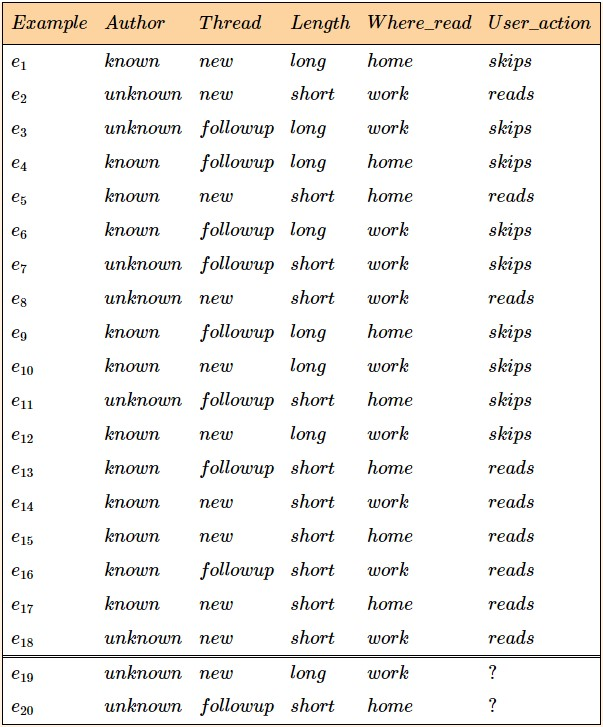
\includegraphics[width=0.55\textwidth]{abc.jpg}
    % \end{figure}



    % \begin{enumerate}
    
    % \item Apresente uma árvore de decisão para a classificação das \textit{User-actions} e calcule o grau de impureza ($I_G$) médio do nó raiz da sua árvore. (Obs: $I_G(p) = 1 - \sum_{i=1}^{J}p_i^2$)
        
    % \item De acordo com a árvore apresentada, qual a classificação dos exemplos $e_{19}$ e $e_{20}$?  
    % \end{enumerate}
    % \end{enumerate}

    
    % \paragraph{Redes Neurais Artificiais}

    % \begin{enumerate}
    %     \item O que é uma rede neural artificial e como ela funciona?

    %     \item Quais são as funções de ativação mais comuns usadas nas redes neurais artificiais e como elas afetam o processo de treinamento?

    %     \item Como o \textit{overfitting} pode ser evitado em redes neurais artificiais?
    % \end{enumerate}



%\bibliographystyle{plain}
%\bibliography{references}

\end{document}
